\begin{figure}
\centering
    \begin{small}

        \begin{verbatim}
    Account:
        int account;
        deposit(int v){
            int temp = account;    #1
            temp = temp + v;
            account = temp;        #2
        }
        withdraw(int v){
            int temp = account;    #3
            temp = temp - v;
            account = temp;        #4
        }
        int inquire(){
            int temp = account;    #5
            return temp;
        }
        \end{verbatim}
        \end{small}
        \caption{A class of \textit{Account}}
        \label{fig:codeaccount}
\end{figure}

\noindent \textbf{Example}
Fig.\ref{fig:codeaccount} is a class of \textit{Account}, which holds an integer $account$ and three operations respectively for increasing, decreasing and reading it. The sentences labeled ``\#'' are considered atomic instructions that access some memory locations.

Fig.\ref{fig:accountcoarsegrain} presents a coarse-grained trace composed of three operations, where $c_1,c_2,c_3$ and $r_1,r_2,r_3$ respectively indicate their invocations and responses. Since neither $r_1\prec c_2$ nor $r_2\prec c_1$, there is no \textit{happen-before} relation between $O_1$ and $O_2$; since $r_2\prec c_3$, then $O_2\sqsubset_S O_3$. \\

%a well-formed coarse-grained trace of a \textit{Set} composed of two operations $O_1$ and $O_2$, and invocation and response events of $O_1 (O_2)$ are $c_1,r_1 (c_2,r_2)$. Since neither $r_1\prec c_2$ nor $r_2\prec c_1$, there is no \textit{happen-before} relation between $O_1$ and $O_2$.

%\begin{figure}
\begin{subfigure}[b]{0.24\textwidth}
    \setlength{\unitlength}{0.5cm}
    \begin{picture}(6.5,2.6)
        \begin{small}
        \put(0,1.7){Thd 1}
        \put(0,0.4){Thd 2}
        \end{small}
        \thinlines
        \multiput(2,1.8)(0.2,0){27}{\line(1,0){0.1}}
        \multiput(2,0.5)(0.2,0){27}{\line(1,0){0.1}}

        \thicklines
        \put(2.3,1.8){\line(1,0){3}}
        \put(3.2,0.5){\line(1,0){3}}

        \put(2.3,1.7){\line(0,1){0.2}}
        \put(3.2,0.4){\line(0,1){0.2}}
        \put(5.3,1.7){\line(0,1){0.2}}
        \put(6.2,0.4){\line(0,1){0.2}}



        \put(2.2,2.1){$c_1$}
        \put(5.2,2.1){$r_1$}
        \put(2.8,0.8){$c_2$}
        \put(5.8,0.8){$r_2$}

        \put(3.7,2.1){$O_1$}
        \put(4.2,0.8){$O_2$}
    \end{picture}
    \caption{A coarse-grained trace}\label{fig:coarsegrainedtrace}
\end{subfigure}
\hfill
\begin{subfigure}[b]{0.24\textwidth}
    \setlength{\unitlength}{0.5cm}
    \begin{picture}(6.5,2.6)
        \begin{small}
        \put(0,1.7){Thd 1}
        \put(0,0.4){Thd 2}
        \end{small}
        \thinlines
        \multiput(2,1.8)(0.2,0){27}{\line(1,0){0.1}}
        \multiput(2,0.5)(0.2,0){27}{\line(1,0){0.1}}

        \thicklines
        \put(2.3,1.8){\line(1,0){3}}
        \put(3.2,0.5){\line(1,0){3}}

        \put(2.3,1.7){\line(0,1){0.2}}
        \put(3.2,0.4){\line(0,1){0.2}}
        \put(5.3,1.7){\line(0,1){0.2}}
        \put(6.2,0.4){\line(0,1){0.2}}



        \put(2.2,2.1){$c_1$}
        \put(5.2,2.1){$r_1$}
        \put(2.8,0.8){$c_2$}
        \put(5.8,0.8){$r_2$}

        \put(3.7,2.1){$O_1$}
        \put(4.2,0.8){$O_2$}
    \end{picture}
    \caption{A coarse-grained trace}\label{fig:coarsegrainedtrace2}
\end{subfigure}

\end{figure}

\begin{figure}
\centering
\setlength{\unitlength}{0.5cm}
    \begin{picture}(16,4)
        \begin{small}
        \put(0,3.8){initial state: \texttt{account = 1}}
        \put(0,2.1){Thread 1}
        \put(0,0.4){Thread 2}
        \end{small}
        \thinlines
        \multiput(2.8,2.2)(0.2,0){65}{\line(1,0){0.1}}
        \multiput(2.8,0.5)(0.2,0){65}{\line(1,0){0.1}}

        \thicklines
        \put(4,2.2){\line(1,0){4}}
        \put(5.4,0.5){\line(1,0){4}}
        \put(10.5,2.2){\line(1,0){4}}

        \put(4,2.1){\line(0,1){0.2}}
        \put(5.4,0.4){\line(0,1){0.2}}
        \put(8,2.1){\line(0,1){0.2}}
        \put(9.4,0.4){\line(0,1){0.2}}
        \put(10.5,2.1){\line(0,1){0.2}}
        \put(14.5,2.1){\line(0,1){0.2}}


        \put(3.8,1.7){$c_1$}
        \put(7.8,1.7){$r_1$}
        \put(5.2,0){$c_2$}
        \put(9.2,0){$r_2$}
        \put(10.3,1.7){$c_3$}
        \put(14.3,1.7){$r_3$}
        \small
        \put(3.8,2.5){$O_1: \mathtt{deposit(1)}$}
        \put(5,0.8){$O_2: \mathtt{withdraw(1)}$}
        \put(9.7,2.5){$O_3: \mathtt{inquire()\to 0}$}
    \end{picture}
    \caption{A coarse-grained trace}\label{fig:accountcoarsegrain}
\end{figure}


\begin{figure}[!ht]
\centering
\includegraphics[width = 3.1in]{atm_1.eps}
\caption{Interleaving tree of the concurrent program}\label{fig:accountintertree}
\end{figure}


\begin{figure}[!ht]
\centering
\includegraphics[width = 3in]{labeledatm.eps}
\caption{Labeled interleaving tree of \textit{Account}}\label{fig:accountlabeledtree}
\end{figure}




